\documentclass[twoside]{book}

% Packages required by doxygen
\usepackage{fixltx2e}
\usepackage{calc}
\usepackage{doxygen}
\usepackage[export]{adjustbox} % also loads graphicx
\usepackage{graphicx}
\usepackage[utf8]{inputenc}
\usepackage{makeidx}
\usepackage{multicol}
\usepackage{multirow}
\PassOptionsToPackage{warn}{textcomp}
\usepackage{textcomp}
\usepackage[nointegrals]{wasysym}
\usepackage[table]{xcolor}

% NLS support packages
\usepackage[french]{babel}

% Font selection
\usepackage[T1]{fontenc}
\usepackage[scaled=.90]{helvet}
\usepackage{courier}
\usepackage{amssymb}
\usepackage{sectsty}
\renewcommand{\familydefault}{\sfdefault}
\allsectionsfont{%
  \fontseries{bc}\selectfont%
  \color{darkgray}%
}
\renewcommand{\DoxyLabelFont}{%
  \fontseries{bc}\selectfont%
  \color{darkgray}%
}
\newcommand{\+}{\discretionary{\mbox{\scriptsize$\hookleftarrow$}}{}{}}

% Page & text layout
\usepackage{geometry}
\geometry{%
  a4paper,%
  top=2.5cm,%
  bottom=2.5cm,%
  left=2.5cm,%
  right=2.5cm%
}
\tolerance=750
\hfuzz=15pt
\hbadness=750
\setlength{\emergencystretch}{15pt}
\setlength{\parindent}{0cm}
\setlength{\parskip}{3ex plus 2ex minus 2ex}
\makeatletter
\renewcommand{\paragraph}{%
  \@startsection{paragraph}{4}{0ex}{-1.0ex}{1.0ex}{%
    \normalfont\normalsize\bfseries\SS@parafont%
  }%
}
\renewcommand{\subparagraph}{%
  \@startsection{subparagraph}{5}{0ex}{-1.0ex}{1.0ex}{%
    \normalfont\normalsize\bfseries\SS@subparafont%
  }%
}
\makeatother

% Headers & footers
\usepackage{fancyhdr}
\pagestyle{fancyplain}
\fancyhead[LE]{\fancyplain{}{\bfseries\thepage}}
\fancyhead[CE]{\fancyplain{}{}}
\fancyhead[RE]{\fancyplain{}{\bfseries\leftmark}}
\fancyhead[LO]{\fancyplain{}{\bfseries\rightmark}}
\fancyhead[CO]{\fancyplain{}{}}
\fancyhead[RO]{\fancyplain{}{\bfseries\thepage}}
\fancyfoot[LE]{\fancyplain{}{}}
\fancyfoot[CE]{\fancyplain{}{}}
\fancyfoot[RE]{\fancyplain{}{\bfseries\scriptsize Généré par Doxygen }}
\fancyfoot[LO]{\fancyplain{}{\bfseries\scriptsize Généré par Doxygen }}
\fancyfoot[CO]{\fancyplain{}{}}
\fancyfoot[RO]{\fancyplain{}{}}
\renewcommand{\footrulewidth}{0.4pt}
\renewcommand{\chaptermark}[1]{%
  \markboth{#1}{}%
}
\renewcommand{\sectionmark}[1]{%
  \markright{\thesection\ #1}%
}

% Indices & bibliography
\usepackage{natbib}
\usepackage[titles]{tocloft}
\setcounter{tocdepth}{3}
\setcounter{secnumdepth}{5}
\makeindex

% Hyperlinks (required, but should be loaded last)
\usepackage{ifpdf}
\ifpdf
  \usepackage[pdftex,pagebackref=true]{hyperref}
\else
  \usepackage[ps2pdf,pagebackref=true]{hyperref}
\fi
\hypersetup{%
  colorlinks=true,%
  linkcolor=blue,%
  citecolor=blue,%
  unicode%
}

% Custom commands
\newcommand{\clearemptydoublepage}{%
  \newpage{\pagestyle{empty}\cleardoublepage}%
}

\usepackage{caption}
\captionsetup{labelsep=space,justification=centering,font={bf},singlelinecheck=off,skip=4pt,position=top}

%===== C O N T E N T S =====

\begin{document}

% Titlepage & ToC
\hypersetup{pageanchor=false,
             bookmarksnumbered=true,
             pdfencoding=unicode
            }
\pagenumbering{alph}
\begin{titlepage}
\vspace*{7cm}
\begin{center}%
{\Large Hg\+P\+OS }\\
\vspace*{1cm}
{\large Généré par Doxygen 1.8.13}\\
\end{center}
\end{titlepage}
\clearemptydoublepage
\pagenumbering{roman}
\tableofcontents
\clearemptydoublepage
\pagenumbering{arabic}
\hypersetup{pageanchor=true}

%--- Begin generated contents ---
\chapter{Hg\+P\+OS}
\label{md__home_yttrium_Documents_Development_HgPOS_README}
\Hypertarget{md__home_yttrium_Documents_Development_HgPOS_README}
Mercure point of sale

\section*{Base de données}

\subsubsection*{Tables concernant la vente et la gestion des stocks}

\subparagraph*{Produits}


\begin{DoxyItemize}
\item {\bfseries id\+Produit}
\item nom
\item prix
\item ico (nom du fichier icone du produit)
\item type
\begin{DoxyItemize}
\item 1 \+: Snacks
\item 2 \+: Boissons
\item 10 \+: Sandwich (unique)
\item 20 \+: Impressions
\item 30 \+: Goodies
\item 40 \+: Adhésion (unique)
\end{DoxyItemize}
\end{DoxyItemize}

\subparagraph*{Stocks}


\begin{DoxyItemize}
\item {\bfseries id\+Stock}
\item {\itshape id\+Produit} (Produits)
\item unite (unites actuels en stock)
\end{DoxyItemize}

\subparagraph*{Ventes}


\begin{DoxyItemize}
\item {\bfseries id\+Vente}
\item {\itshape id\+Produit} (Produits)
\item unite (unites vendues)
\end{DoxyItemize}

\subparagraph*{Formules}


\begin{DoxyItemize}
\item {\bfseries id\+Formule}
\item {\itshape id\+Produit\+Sandwich} (Produits)
\item {\itshape id\+Produit\+Snack} (Produits)
\item {\itshape id\+Produit\+Boisson} (Produits)
\end{DoxyItemize}

\subsubsection*{Autres tables}

\paragraph*{Membres}


\begin{DoxyItemize}
\item {\bfseries id\+Membre}
\item nom
\item prenom
\item email
\item statut
\begin{DoxyItemize}
\item L1
\item L2M
\item L3M
\item M1M
\item M2M
\item L2I
\item L3I
\item M1I
\item M2I
\item A\+U\+T\+RE
\end{DoxyItemize}
\end{DoxyItemize}

\paragraph*{Utilisateurs}


\begin{DoxyItemize}
\item {\bfseries id\+Utilisateur}
\item nom
\item mdp
\item droits 
\end{DoxyItemize}
\chapter{Index hiérarchique}
\section{Hiérarchie des classes}
Cette liste d\textquotesingle{}héritage est classée approximativement par ordre alphabétique \+:\begin{DoxyCompactList}
\item \contentsline{section}{Database\+Manager}{\pageref{classDatabaseManager}}{}
\item \contentsline{section}{Panier}{\pageref{classPanier}}{}
\item \contentsline{section}{Produit}{\pageref{classProduit}}{}
\item Q\+Main\+Window\begin{DoxyCompactList}
\item \contentsline{section}{Main\+Window}{\pageref{classMainWindow}}{}
\end{DoxyCompactList}
\end{DoxyCompactList}

\chapter{Index des classes}
\section{Liste des classes}
Liste des classes, structures, unions et interfaces avec une brève description \+:\begin{DoxyCompactList}
\item\contentsline{section}{\hyperlink{classDatabaseManager}{Database\+Manager} \\*The \hyperlink{classDatabaseManager}{Database\+Manager} class La class est utilisé pour accéder à la base de données sqlite }{\pageref{classDatabaseManager}}{}
\item\contentsline{section}{\hyperlink{classMainWindow}{Main\+Window} \\*The \hyperlink{classMainWindow}{Main\+Window} class La class pour la fenêtre principale }{\pageref{classMainWindow}}{}
\item\contentsline{section}{\hyperlink{classPanier}{Panier} }{\pageref{classPanier}}{}
\item\contentsline{section}{\hyperlink{classProduit}{Produit} \\*Class représentant un produit }{\pageref{classProduit}}{}
\end{DoxyCompactList}

\chapter{Documentation des classes}
\hypertarget{classDatabaseManager}{}\section{Référence de la classe Database\+Manager}
\label{classDatabaseManager}\index{Database\+Manager@{Database\+Manager}}


The \hyperlink{classDatabaseManager}{Database\+Manager} class La class est utilisé pour accéder à la base de données sqlite.  




{\ttfamily \#include $<$databasemanager.\+h$>$}

\subsection*{Fonctions membres publiques}
\begin{DoxyCompactItemize}
\item 
\mbox{\Hypertarget{classDatabaseManager_aa162d97472e6c31a4e873adda435dbb6}\label{classDatabaseManager_aa162d97472e6c31a4e873adda435dbb6}} 
\hyperlink{classDatabaseManager_aa162d97472e6c31a4e873adda435dbb6}{Database\+Manager} ()
\begin{DoxyCompactList}\small\item\em \hyperlink{classDatabaseManager_aa162d97472e6c31a4e873adda435dbb6}{Database\+Manager\+::\+Database\+Manager} Crée la connexion avec la base de données. \end{DoxyCompactList}\item 
\mbox{\Hypertarget{classDatabaseManager_ae9b3a5da1e04fbb00faf8a034da1d063}\label{classDatabaseManager_ae9b3a5da1e04fbb00faf8a034da1d063}} 
\hyperlink{classDatabaseManager_ae9b3a5da1e04fbb00faf8a034da1d063}{$\sim$\+Database\+Manager} ()
\begin{DoxyCompactList}\small\item\em \hyperlink{classDatabaseManager_ae9b3a5da1e04fbb00faf8a034da1d063}{Database\+Manager\+::$\sim$\+Database\+Manager}. \end{DoxyCompactList}\item 
Q\+List$<$ \hyperlink{classProduit}{Produit} $>$ $\ast$ \hyperlink{classDatabaseManager_a00bdab5cbbf85a15d297706509b474af}{get\+Produit\+List} ()
\begin{DoxyCompactList}\small\item\em \hyperlink{classDatabaseManager_a00bdab5cbbf85a15d297706509b474af}{Database\+Manager\+::get\+Produit\+List}. \end{DoxyCompactList}\end{DoxyCompactItemize}


\subsection{Description détaillée}
The \hyperlink{classDatabaseManager}{Database\+Manager} class La class est utilisé pour accéder à la base de données sqlite. 

\subsection{Documentation des fonctions membres}
\mbox{\Hypertarget{classDatabaseManager_a00bdab5cbbf85a15d297706509b474af}\label{classDatabaseManager_a00bdab5cbbf85a15d297706509b474af}} 
\index{Database\+Manager@{Database\+Manager}!get\+Produit\+List@{get\+Produit\+List}}
\index{get\+Produit\+List@{get\+Produit\+List}!Database\+Manager@{Database\+Manager}}
\subsubsection{\texorpdfstring{get\+Produit\+List()}{getProduitList()}}
{\footnotesize\ttfamily Q\+List$<$ \hyperlink{classProduit}{Produit} $>$ $\ast$ Database\+Manager\+::get\+Produit\+List (\begin{DoxyParamCaption}{ }\end{DoxyParamCaption})}



\hyperlink{classDatabaseManager_a00bdab5cbbf85a15d297706509b474af}{Database\+Manager\+::get\+Produit\+List}. 

\begin{DoxyReturn}{Renvoie}
liste des produits (icon chargés) 
\end{DoxyReturn}


La documentation de cette classe a été générée à partir des fichiers suivants \+:\begin{DoxyCompactItemize}
\item 
/home/yttrium/\+Documents/\+Development/\+Hg\+P\+O\+S/databasemanager.\+h\item 
/home/yttrium/\+Documents/\+Development/\+Hg\+P\+O\+S/databasemanager.\+cpp\end{DoxyCompactItemize}

\hypertarget{classMainWindow}{}\section{Référence de la classe Main\+Window}
\label{classMainWindow}\index{Main\+Window@{Main\+Window}}


The \hyperlink{classMainWindow}{Main\+Window} class La class pour la fenêtre principale.  




{\ttfamily \#include $<$mainwindow.\+h$>$}

Graphe d\textquotesingle{}héritage de Main\+Window\+:\begin{figure}[H]
\begin{center}
\leavevmode
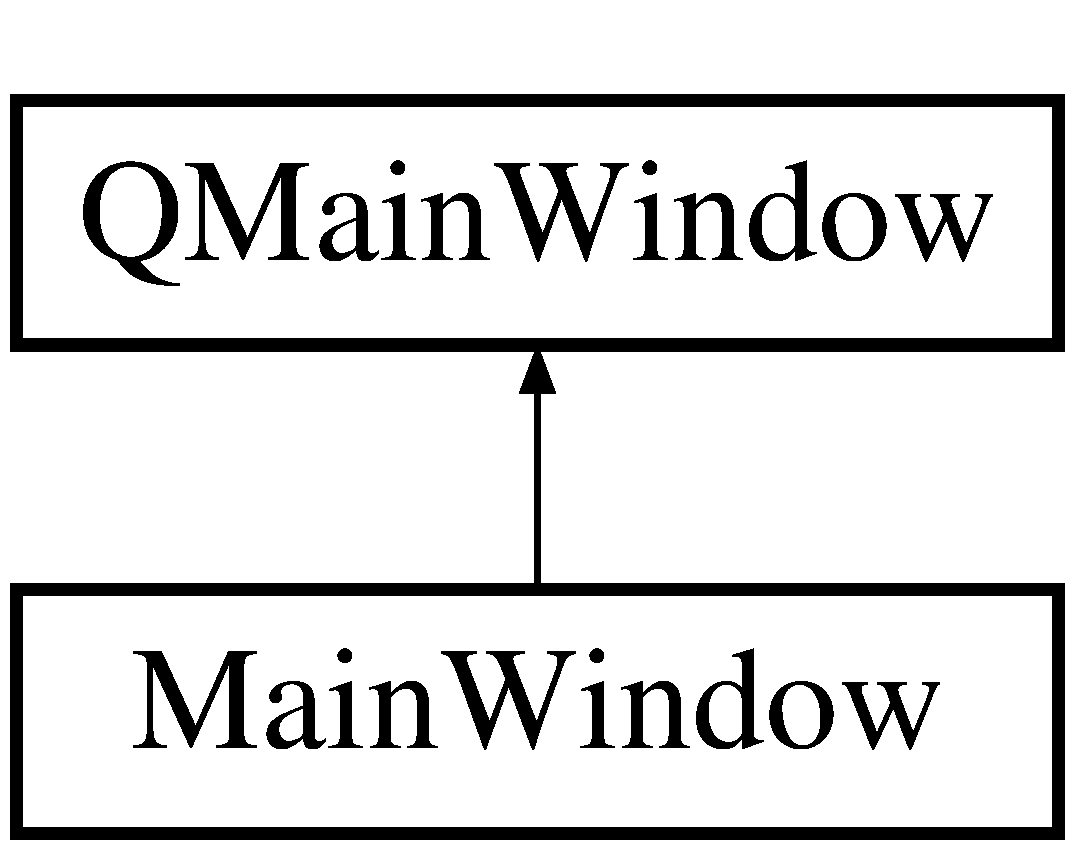
\includegraphics[height=2.000000cm]{classMainWindow}
\end{center}
\end{figure}
\subsection*{Fonctions membres publiques}
\begin{DoxyCompactItemize}
\item 
\mbox{\Hypertarget{classMainWindow_a8b244be8b7b7db1b08de2a2acb9409db}\label{classMainWindow_a8b244be8b7b7db1b08de2a2acb9409db}} 
{\bfseries Main\+Window} (Q\+Widget $\ast$parent=0)
\end{DoxyCompactItemize}


\subsection{Description détaillée}
The \hyperlink{classMainWindow}{Main\+Window} class La class pour la fenêtre principale. 

La documentation de cette classe a été générée à partir des fichiers suivants \+:\begin{DoxyCompactItemize}
\item 
/home/yttrium/\+Documents/\+Development/\+Hg\+P\+O\+S/mainwindow.\+h\item 
/home/yttrium/\+Documents/\+Development/\+Hg\+P\+O\+S/mainwindow.\+cpp\item 
/home/yttrium/\+Documents/\+Development/\+Hg\+P\+O\+S/mainwindowslots.\+cpp\end{DoxyCompactItemize}

\hypertarget{classPanier}{}\section{Référence de la classe Panier}
\label{classPanier}\index{Panier@{Panier}}
\subsection*{Fonctions membres publiques}
\begin{DoxyCompactItemize}
\item 
\mbox{\Hypertarget{classPanier_adc423444697a339bed7ba2e68eab3d21}\label{classPanier_adc423444697a339bed7ba2e68eab3d21}} 
void \hyperlink{classPanier_adc423444697a339bed7ba2e68eab3d21}{clear} ()
\begin{DoxyCompactList}\small\item\em clear efface le panier actuel. \end{DoxyCompactList}\end{DoxyCompactItemize}
\subsection*{Attributs publics}
\begin{DoxyCompactItemize}
\item 
\mbox{\Hypertarget{classPanier_a8f5aa56eb718268b34ce98c1c6f355d0}\label{classPanier_a8f5aa56eb718268b34ce98c1c6f355d0}} 
Q\+List$<$ \hyperlink{classProduit}{Produit} $>$ \hyperlink{classPanier_a8f5aa56eb718268b34ce98c1c6f355d0}{prod}
\begin{DoxyCompactList}\small\item\em prod, la liste des produits dans le panier \end{DoxyCompactList}\item 
\mbox{\Hypertarget{classPanier_ad7c7bd79f43a8686805302d091207e64}\label{classPanier_ad7c7bd79f43a8686805302d091207e64}} 
Q\+List$<$ unsigned int $>$ \hyperlink{classPanier_ad7c7bd79f43a8686805302d091207e64}{unit}
\begin{DoxyCompactList}\small\item\em unit, la liste du nombre d\textquotesingle{}unité de produits dans le panier \end{DoxyCompactList}\end{DoxyCompactItemize}


La documentation de cette classe a été générée à partir du fichier suivant \+:\begin{DoxyCompactItemize}
\item 
/home/yttrium/\+Documents/\+Development/\+Hg\+P\+O\+S/panier.\+h\end{DoxyCompactItemize}

\hypertarget{classProduit}{}\section{Référence de la classe Produit}
\label{classProduit}\index{Produit@{Produit}}


Class représentant un produit.  




{\ttfamily \#include $<$produit.\+h$>$}

\subsection*{Attributs publics}
\begin{DoxyCompactItemize}
\item 
\mbox{\Hypertarget{classProduit_ad999fe48d24e14d6779a9f03eb5f9b97}\label{classProduit_ad999fe48d24e14d6779a9f03eb5f9b97}} 
int {\bfseries id\+Produit}
\item 
\mbox{\Hypertarget{classProduit_a582becfbc8aef72c99f83a37642cf7a5}\label{classProduit_a582becfbc8aef72c99f83a37642cf7a5}} 
Q\+String {\bfseries nom}
\item 
\mbox{\Hypertarget{classProduit_a42ef1d4887be85e601553ad082096263}\label{classProduit_a42ef1d4887be85e601553ad082096263}} 
float {\bfseries prix}
\item 
\mbox{\Hypertarget{classProduit_a688a2383686260a3b2f3b7d51cd2d2e4}\label{classProduit_a688a2383686260a3b2f3b7d51cd2d2e4}} 
Q\+String {\bfseries ico}
\item 
\mbox{\Hypertarget{classProduit_ac7b21ab414deecfc386addacf78e1bea}\label{classProduit_ac7b21ab414deecfc386addacf78e1bea}} 
Q\+Icon {\bfseries qicon}
\item 
\mbox{\Hypertarget{classProduit_a193fb38f5b87fae05474a35e6c7a905c}\label{classProduit_a193fb38f5b87fae05474a35e6c7a905c}} 
int {\bfseries type}
\end{DoxyCompactItemize}


\subsection{Description détaillée}
Class représentant un produit. 

La documentation de cette classe a été générée à partir du fichier suivant \+:\begin{DoxyCompactItemize}
\item 
/home/yttrium/\+Documents/\+Development/\+Hg\+P\+O\+S/produit.\+h\end{DoxyCompactItemize}

%--- End generated contents ---

% Index
\backmatter
\newpage
\phantomsection
\clearemptydoublepage
\addcontentsline{toc}{chapter}{Index}
\printindex

\end{document}
